\documentclass[english]{article}
\usepackage[T1]{fontenc}
%\usepackage[latin9]{inputenc}
%\usepackage{geometry}
%\geometry{verbose,tmargin=1in,bmargin=1in,lmargin=1in,rmargin=1in}
\usepackage{amsmath}
\usepackage{amssymb}
\usepackage{setspace}
\usepackage[utf8]{inputenc}
\usepackage{graphicx}
\usepackage{float}
\usepackage{adjustbox}
\usepackage{gensymb}
\usepackage{amssymb}
\usepackage{array}
\usepackage{ragged2e}
\usepackage{lipsum}
\onehalfspacing
\usepackage{babel}
\usepackage{tikz}
\usepackage{ctable}
\usepackage{booktabs}
\usepackage{graphicx}
\usepackage{caption}
\usepackage{placeins}
\usepackage{todonotes}
\usepackage{subcaption}
\usepackage[font=footnotesize,labelformat=simple]{subcaption}
\usepackage[T1]{fontenc}
\usepackage{pdflscape}
\usepackage{blindtext}
\usepackage{parskip}
\setlength{\parskip}{16pt}

\begin{document}

\title{Informality in LAC: Heterogeneity and Disappointing Progress}
\maketitle
\begin{abstract}

    This descriptive paper uses household and employment surveys from the Latin America and the Caribbean region to paint a more complete picture of the different aspects of informality. We start by discussing alternative informality measures at the regional and cross country level. We then show that there has been progress on increasing the share of dependent workers who contribute to social security but that the productive structure of the economies in the region has remained mostly unchanged. We argue that this is mainly coming from the focus of governments policies on facilitating the registration of low productivity workers, therefore subsidizing low productivity firms. To make this point we use two approaches: a qualitative approach based on the analysis of policies that have been identified as successful in reducing informality. Second, we use a simple decomposition on different formalization margins to show that the formalization process in the region has been dominated by workers transitioning to formal status in the same type of firm. This means that the progress made in formalizing workers has happened mainly through increasing coverage of workers in small firms. 
\end{abstract}

\section{Introduction}

Informality remains a pervasive and challenging problem in labor markets across many regions, despite numerous policy interventions aimed at reducing it. The issue persists as a central concern due to its significant implications for economic development, social protection, and labor rights. In many developing countries, informality represents a sizable portion of the labor market, affecting millions of workers who operate outside the boundaries of formal legal protections. The phenomenon of informality is multi-faceted, encompassing a variety of employment arrangements that fail to conform to established labor laws and regulations, leaving workers vulnerable and without access to essential social protections.

Motivation for examining informality stems from the recognition that, despite widespread attempts to curtail it, informality continues to undermine progress toward inclusive and sustainable development. The persistence of informality is particularly concerning in regions with high levels of inequality and poverty, where formal employment opportunities remain scarce, and many workers are forced to rely on informal jobs as their primary source of income. Understanding the nature of informality, its causes, and the barriers to reducing it is essential for crafting effective policies that can bring more workers into the formal economy, protect their rights, and improve their livelihoods.

The discussion around informality has evolved over time, reflecting changing economic conditions, labor market dynamics, and policy priorities. One of the most widely recognized definitions of informality comes from the International Labour Organization (ILO), which seeks to capture and compare related but distinct phenomena that contribute to the complexity of informal employment. The ILO’s definition of informality encompasses several key aspects:

Informal workers and enterprises are often characterized by low levels of productivity, limited access to capital, technology, and skills, and are frequently excluded from formal financial and business support systems.
Unprotected workers: Informal employment typically involves a lack of social protection, including access to healthcare, pensions, unemployment insurance, and other forms of labor security, leaving workers exposed to economic shocks and personal risks.

Informal work may also involve non-compliance with labor laws and regulations, including minimum wage standards, occupational health and safety norms, and working hour limitations, further exacerbating the vulnerability of workers in these sectors. While these dimensions of informality are interrelated, they capture different aspects of a broader phenomenon, and policies targeting one area may not necessarily address the others. As such, understanding the full scope of informality requires a nuanced approach that recognizes its diversity and complexity.

One of the central arguments of this paper is that informality is not a uniform or static phenomenon; rather, it is dynamic and shaped by a range of factors, including economic conditions, institutional frameworks, and individual worker characteristics. Informal employment varies significantly across different sectors, demographic groups, and geographic regions, requiring tailored policy responses that account for these differences. In some cases, informality arises from necessity, as workers are unable to find formal jobs, while in others, it may reflect a preference for more flexible or autonomous work arrangements.

In addition to these variations, informality can take different forms depending on the level of development and the structure of the economy. For instance, in rural areas, informality is often associated with small-scale agricultural production and family businesses, while in urban centers, it may be linked to low-wage service sector jobs or self-employment in unregulated markets. These distinctions are important for policymakers seeking to design interventions that can effectively target the root causes of informality and support workers in transitioning to formal employment.

The evolution of informality in the region over the past two decades suggests that progress is possible, but it requires sustained effort and coordination across multiple sectors of the economy. While many countries have made strides in reducing informality, particularly through labor market formalization and social protection expansion, the informal economy remains a significant challenge. This paper aims to provide a deeper understanding of informality by critically examining its definition, analyzing the progress made in reducing it, and reviewing the policy efforts undertaken to address it.

This paper is divided into two main sections. The first section delves into the mainstream definition of informality as presented by the ILO and other international organizations. It looks "under the hood" of this definition, exploring the evolution of alternative measures of informality and efforts to categorize and characterize different segments of the informal economy. The section also documents the progress that has been made in reducing informality in the region over the last two decades. Despite these advances, informal employment remains a stubborn issue, and the analysis will focus on the varying margins of progress across different countries and economic sectors. By examining the trajectory of informality in this context, the section seeks to provide a more granular understanding of where and how informality has been reduced, and where significant challenges remain.

The second section shifts focus to the policy landscape, offering a comprehensive summary of the reforms that have been implemented across the region with the explicit goal of reducing informality. Over the years, countries have adopted a variety of strategies aimed at formalizing employment, including labor market reforms, social protection programs, and regulatory adjustments. This section provides an overview of these reforms, evaluating their impact on the labor market and assessing their effectiveness in curbing informality. While some reforms have been successful in bringing workers into the formal economy, others have faced significant implementation challenges or have failed to reach their intended targets. The discussion will highlight key lessons learned from these reform efforts, as well as the factors that have contributed to their success or failure.

By providing a comprehensive overview of the current state of informality and the policies aimed at reducing it, this paper contributes to the ongoing debate about how best to tackle informal employment and ensure that workers across the region have access to decent work and social protection. Through a detailed examination of the progress and challenges in this area, the paper seeks to inform future policy decisions and encourage more targeted and effective approaches to reducing informality.


\section{Complexity of Informality}

The concept of informality has a long and complex history, evolving in both its theoretical foundations and practical implications over time. From its early theoretical roots in the 1970s to the wide-ranging debates on its definition and scope today, informality has emerged as a significant challenge for policymakers, particularly in developing regions. Its persistent and multifaceted nature, encompassing issues of productivity, worker protection, and regulatory non-compliance, demands a more nuanced understanding. In this section, we explore the historical development of the term, the mainstream definition established by international organizations, and the evolving discourse surrounding informality, particularly in regional contexts.

The term "informality" gained prominence in economic literature with the work of Harris and Todaro (1970), who introduced the idea that informal employment serves as a buffer for workers unable to find formal sector jobs. Their dual-sector model, which described rural-urban migration and urban unemployment, set the stage for understanding informal employment as a response to limited opportunities in the formal economy. In their model, individuals migrate to urban areas expecting higher wages in formal employment but, unable to secure such jobs, they engage in informal work as a survival strategy.

The conceptualization of informality was further expanded by Hernando De Soto in the 1980s, who emphasized the role of excessive regulation and bureaucratic barriers in pushing workers and enterprises into the informal sector. De Soto argued that informal workers and businesses were not inherently inefficient but were rather driven into informality by structural obstacles within the formal system. His work suggested that informality was, in part, a response to state-imposed constraints, and that reforms aimed at reducing regulatory burdens could help formalize much of the informal economy.

More recent literature, such as the work of Perry et al. and Ulyssea (2017), has expanded on these early frameworks by examining the heterogeneity of informality and the different motivations behind informal employment. Ulyssea, for example, provides an in-depth analysis of the trade-offs faced by firms and workers in deciding whether to operate formally or informally, emphasizing that informality is not a monolithic category but a complex mix of voluntary and involuntary choices. This growing body of research has deepened our understanding of the informal sector, highlighting that workers and firms may choose informality not just out of necessity but sometimes as a deliberate strategy to avoid costs associated with formality.

The International Labour Organization (ILO) has been instrumental in developing a standardized definition of informality that is widely used in academic and policy discussions today. The ILO defines informal employment as encompassing all forms of work that are not regulated or protected by legal frameworks. This includes workers who do not have access to social protections such as health insurance, pensions, and unemployment benefits, as well as firms that operate outside of legal regulations regarding wages, taxes, and labor standards.

The ILO’s definition distinguishes between informal workers and informal enterprises, creating a matrix that identifies the different dimensions of informality. On the one hand, informal workers include both salaried employees and self-employed individuals who lack formal labor protections, while on the other hand, informal enterprises refer to businesses that are not registered or do not comply with regulatory requirements. The ILO’s approach provides a comprehensive framework for understanding the various forms that informality can take, ranging from unregistered microenterprises to workers in formal firms who are not provided with social protection.

At the ILO’s International Conference of Labour Statisticians (ICLS), these definitions have been continually refined to address growing concerns about the scope of informal employment and the difficulty in capturing it accurately in labor statistics. The most pressing issue that emerged from these meetings was the need to account for the diverse conditions that give rise to informality, from outright evasion of regulations to more structural barriers that prevent workers from accessing formal employment opportunities. Concerns were raised about the role of social protection—particularly the lack of social security coverage—as one of the primary indicators of informality.

Indeed, one of the most significant contributions of the ILO’s definition is the emphasis on social security coverage as a key marker of informal employment. Workers who are not enrolled in social security schemes are considered informal, regardless of other conditions of their employment. This focus highlights the broader social and economic vulnerabilities of informal workers, who are excluded from safety nets that could provide them with protection against income shocks, illness, or old age.

While the ILO’s definition provides a broad framework, it is essential to disaggregate the concept to understand the different types of informality and the specific challenges they pose. At its core, informality can be broken down into three primary components: low productivity, unprotected workers, and unlawful employment. Each of these elements captures a distinct aspect of the informal economy:
\begin{itemize}
\item Low Productivity: Informal enterprises often operate with low levels of productivity due to limited access to capital, technology, and skilled labor. These businesses tend to be small, family-run operations with little potential for growth. This type of informality is particularly prevalent in sectors like agriculture and street vending.

 \item Unprotected Workers: A defining feature of informal employment is the lack of social protection for workers. These individuals are typically excluded from health insurance, pensions, and other benefits that formal workers receive. The absence of social security explains much of the informality in regions where labor markets are segmented and formal job opportunities are scarce.

 \item Unlawful Employment: Informal work often occurs in violation of labor laws and regulations, such as minimum wage laws or working hour limitations. In some cases, employers may deliberately hire workers informally to avoid paying taxes or complying with labor standards, contributing to the persistence of informality.
   
\end{itemize}


Several international organizations have contributed to the discourse on informality through flagship reports that examine the causes, consequences, and potential solutions for this issue. The World Bank (2021), for instance, highlighted the importance of addressing the shadow economy in its efforts to promote economic development. Similarly, the OECD, ILO, and Inter-American Development Bank (IDB) have all produced influential reports that underscore the significance of reducing informality as a means of fostering inclusive growth.

These paper consistently portray informality as a major barrier to development, particularly in regions where formal job opportunities are limited, and regulatory environments are weak. The OECD has focused on the role of labor market institutions and their failure to integrate informal workers, while the IDB has emphasized the importance of social protection programs in bringing workers into the formal sector. Across these analyses, informality is depicted as a public enemy that undermines both economic efficiency and social equity.

In Latin America and other developing regions, the discussion on informality has been particularly robust. Policymakers and researchers alike have framed informality as a critical challenge that must be addressed to improve living standards and foster more inclusive economies. The regional discourse often portrays informality as a structural issue that reflects deeper problems within the labor market, including inequality, insufficient formal job creation, and weak institutions.

The persistence of informality in the region has led to a growing recognition of the need for comprehensive reforms that address the root causes of informality. These include regulatory reforms aimed at simplifying business registration processes, expanding social protection coverage to informal workers, and enhancing labor market institutions to provide better enforcement of labor laws.

In the next section, we take a closer look at the individual components of informality—low productivity, unprotected workers, and unlawful employment—and relate each component to the main policy concerns driving efforts to reduce informality in the region. Through this lens, we can better understand the complex dynamics that perpetuate informality and the targeted solutions required to address them effectively.

\section{Labor Market Structure of the Average LAC Country}

The labor market in Latin America and the Caribbean (LAC) presents a complex and multifaceted structure, shaped by historical legacies, socio-economic inequalities, and persistent informality. While the region has made strides in labor market reforms, it remains characterized by segmentation between formal and informal employment, diverse labor market outcomes based on education levels, firm size, and sectoral distribution. Understanding the structure of the labor market in the average LAC country is essential to grasp the barriers and opportunities for workers across various demographics, particularly in relation to social protection and economic mobility.

This section explores the key dimensions that define the structure of employment in the region, examining the relative distribution of salaried, self-employed, and non-salaried workers. It further dissects employment patterns according to education, firm size, and sectors, providing a comprehensive overview of the dynamics that drive labor market informality and inequality. The analysis will reveal how the prevalence of low-skilled, self-employed, and informal workers affects social security coverage, income security, and productivity in LAC economies. Moreover, it will shed light on the structural barriers that limit access to formal employment, particularly for marginalized groups, and the role of public policy in addressing these challenges.

By outlining these core features, this section aims to provide an insightful understanding of the labor market structure in LAC countries, offering a foundation for policy discussions on improving labor market inclusion, formality, and the overall well-being of workers.

\begin{enumerate}
    \item\textit{Structure of the labor market } 

Figures \ref{fig:labmarket1} and \ref{fig:labmarket2} shows the structure of the labor market for the average Latin American country. It illustrates labor market trends, including gender disparities in participation and unemployment, educational limitations in the workforce, and general employment challenges. Provides critical insight into the demographic composition and labor market conditions of a given country. The chart is separated into two main components: (a) Demographic and (b) Labor market.

\begin{enumerate}
    \item\textit{Demographic}

Age Distribution (25-54 and 18-65 years old):
The proportion of the population aged 25-54 years old is 38.8\%, while the proportion of those between 18 and 65 is 60.4\%. This suggests that the younger workforce (those under 54) makes up a significant part of the overall working-age population, which has implications for both labor market participation and potential productivity. The age structure is critical for understanding labor market dynamics since younger workers often have higher employment prospects, while older workers may face different job market challenges.

Labor Force Participation Rate (18-65 years old):
The participation rate for the broader working-age group (18-65) is 73.3\%, which indicates a robust level of economic engagement. This metric refers to the share of the population in this age bracket that is either employed or actively seeking employment. Such a high participation rate suggests an active labor market but can also highlight areas where unemployment or underemployment might be prevalent.

Female Labor Force Participation:
Female labor force participation is significantly lower than the overall participation rate, standing at 60.4\%. This figure points to gender disparities in labor market engagement. Understanding the drivers of these differences, such as access to education, cultural norms, childcare responsibilities, or discrimination, is essential for policy recommendations aimed at improving gender equality in the workforce.

Additionally, the figure includes minimum and maximum values for each indicator (represented by blue dots for minimum and red squares for maximum), illustrating variability within the data, possibly across different regions or time periods.


 \item\textit{Labor Market}

Labor Force with Tertiary Education:
Only 15\% of the labor force aged 18-65 has attained tertiary education, indicating that a large portion of the workforce may be limited to jobs requiring lower skill levels. This statistic underscores a challenge in raising productivity and moving workers into higher-paying, more formalized sectors. Investment in education and vocational training could play a vital role in shifting workers from low-skilled, informal sectors to more formal employment.

Unemployment Rate:
The overall unemployment rate is 7.6\%, which reflects a moderate level of joblessness. While not excessively high, it still indicates a portion of the labor force is struggling to find employment, which could be related to structural issues, skill mismatches, or economic volatility. Additionally, the maximum unemployment rate, as indicated by the red square, suggests that in some regions or among specific subgroups, unemployment can reach much higher levels.

Female Unemployment:
Female unemployment is higher than the overall unemployment rate, at 9.3\%, signaling gender-specific challenges in accessing employment. These disparities may be the result of factors such as discrimination, gender role expectations, or uneven access to opportunities and training. The relatively higher unemployment among women compared to men suggests a gender imbalance that policymakers need to address, particularly if they are aiming to reduce overall unemployment and foster more inclusive economic growth.

\end{enumerate}
    
\begin{figure}[h!tbp]
\justifying
  \caption{Demographic profile and structure of labor market}
\begin{subfigure}{.9\textwidth}
  \centering
    \subcaption{Demographic}
  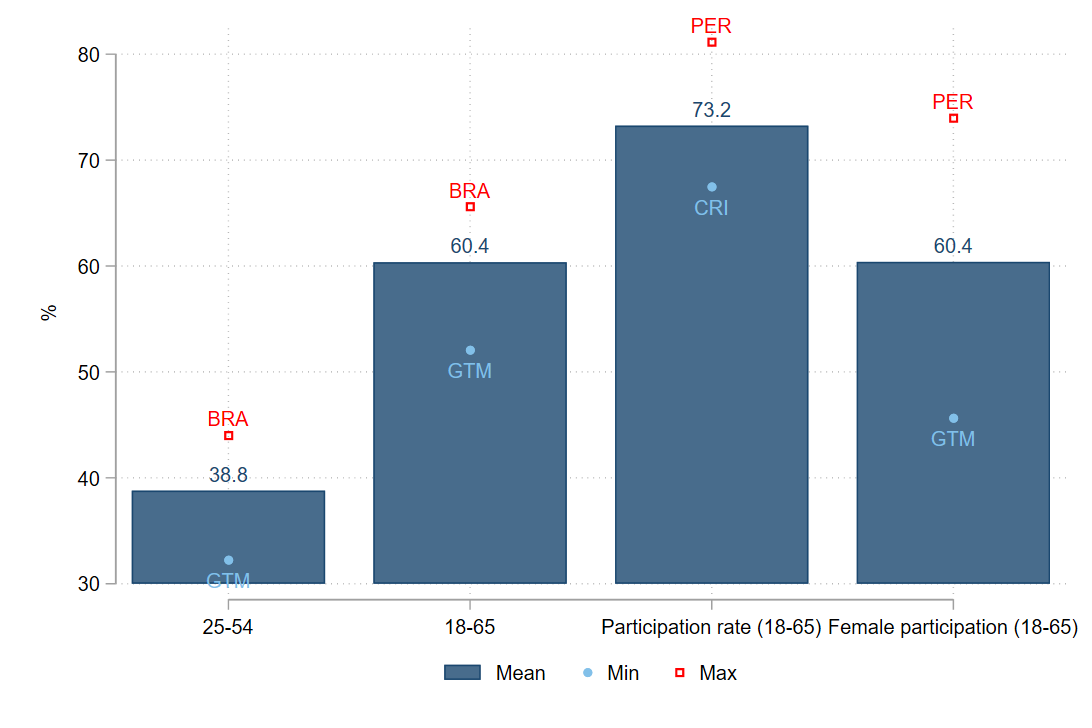
\includegraphics[width=1\linewidth]{latex/figures/Snapshot/Structure of labor market_a.png}
  \label{fig:labmarket1}
\end{subfigure}

\begin{subfigure}{.9\textwidth}
  \centering
    \subcaption{Labor market}
  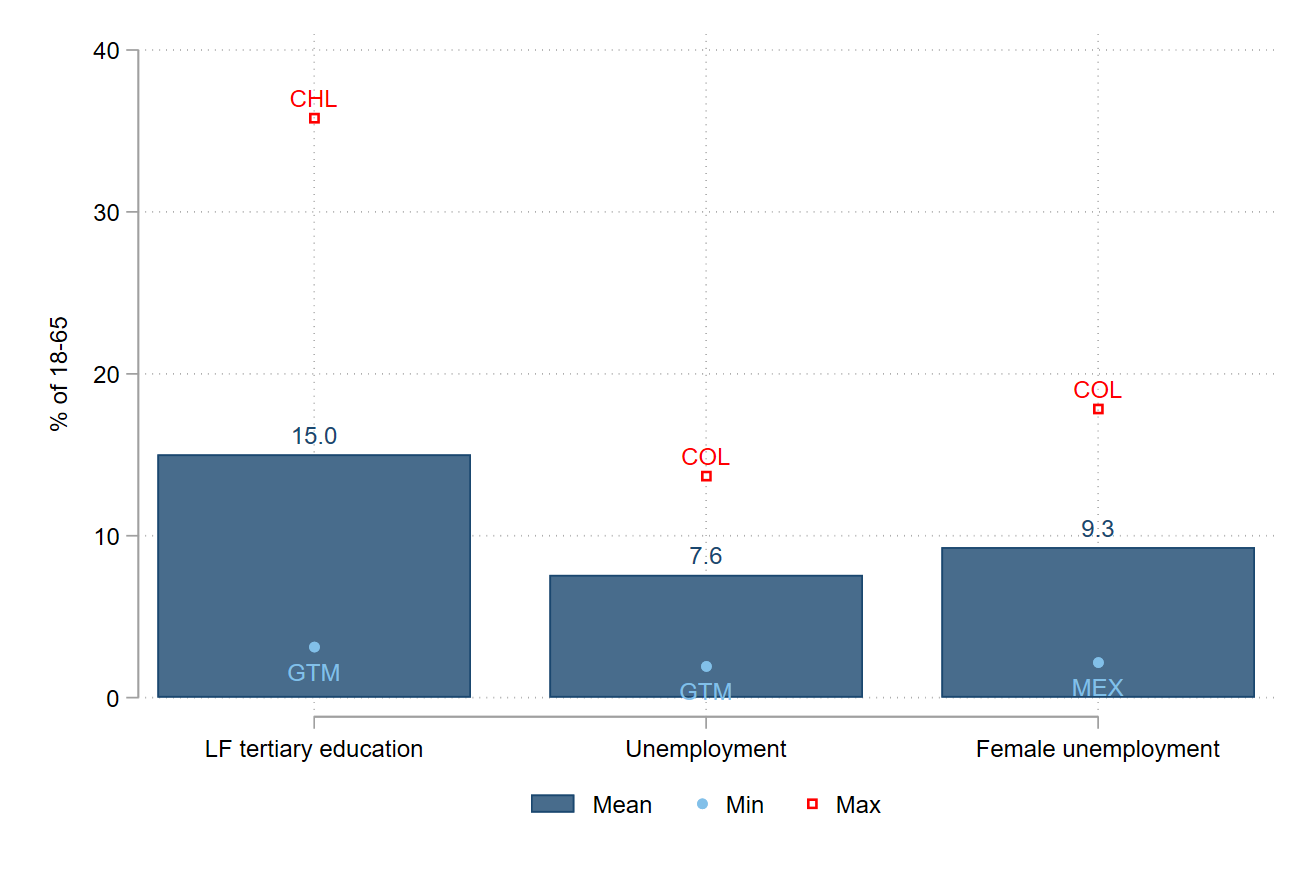
\includegraphics[width=1\linewidth]{latex/figures/Snapshot/Structure of labor market_b.png}
  \label{fig:labmarket2}
\end{subfigure}

\footnotesize{Source: Household Surveys-SEDLAC.}
\footnotesize{Note: Each bar is a simple average of country level weighted average in 2021. Countries included in the sample: Argentina, Bolivia, Brazil, Chile, Colombia, Costa Rica, Dominican Republic, Ecuador, El Salvador, Guatemala, Honduras, Mexico, Panama, Peru, Paraguay and Uruguay. Some countries don’t have information for 2021, in that cases we use the last available year, for Chile 2022, Guatemala 2014; Honduras 2019; Mexico 2018 and Uruguay 2019. Panel a: bar one and two are defined as percentage of the population. Also, "Participation rate" and "Female participation" are define as part of the labor force defined for people between 18 and 65 years old. Panel b: "LF tertiary education" corresponds to people in the workforce who have completed tertiary education.}

\end{figure}


The demographic and labor market profile depicted in this figure reflects many common challenges seen in developing or transitioning economies. A large proportion of the workforce is within prime working age, but the labor force participation rate is skewed toward males, and women’s participation remains significantly lower. These gender disparities indicate structural and cultural barriers, which have important implications for policy aimed at fostering inclusive economic development.

From an educational perspective, the low percentage of workers with tertiary education (15\%) highlights a key constraint in achieving economic growth and reducing informality. Studies on informality, such as Ulyssea (2017), underscore how educational deficits keep workers trapped in low-productivity, informal jobs. Without improving access to higher education or vocational training, efforts to formalize the labor market and boost productivity will be limited.

Unemployment levels, while moderate overall, present regional and gender disparities. Higher female unemployment suggests that gender-specific interventions are necessary to ensure equal access to employment opportunities. Initiatives such as flexible work arrangements, targeted job training for women, and policies to combat workplace discrimination could mitigate these gender gaps in employment. Furthermore, addressing the broader unemployment issue requires understanding the mismatch between the skills offered by workers and the demands of employers.

This figure also invites a deeper discussion on how informality interacts with these labor market indicators. High female unemployment, coupled with lower educational attainment and labor force participation, may lead many women into informal jobs where social protections and legal rights are limited. Similarly, lower-skilled workers with no tertiary education are likely over-represented in informal sectors. The Harris-Todaro model (1970) of urban unemployment provides insights into how migration from rural to urban areas, in search of better opportunities, can exacerbate informal labor market growth if formal job creation is insufficient.

Flagship reports from international organizations such as the World Bank, the OECD, and the ILO emphasize the need for comprehensive labor reforms to address these structural issues. These reforms should focus on improving educational outcomes, promoting gender equality, and creating more formal employment opportunities, particularly for vulnerable groups.


\item\textit{Structure of Employment}

The structure of employment in Latin America reveals the central challenge of labor informality, with significant portions of the workforce engaged in self-employment and non-salaried work. While salaried employment remains the dominant form of employment, the heterogeneity across countries and employment types underscores the need for tailored policy responses. Addressing informality requires a focus on educational investments, entrepreneurial support, and inclusive labor regulations that ensure all workers, regardless of their employment status, can access social protections and fair working conditions. This multi-faceted approach will be critical for promoting inclusive economic growth and reducing labor market segmentation across the region.

The figure \ref{fig:employment} illustrates the employment distribution across four key categories: salaried employment, self-employment, employers, and non-salaried workers. The data is derived from household surveys and represents the weighted average across several Latin American countries in 2021. This section provides a detailed academic analysis of the structure of employment, drawing on the information presented in the graph and connecting it with broader discussions on labor informality and economic structure.

The largest proportion of employment is concentrated in salaried positions, representing 61.5\% of the labor force. This category typically includes formal employment, where workers receive a regular wage or salary and are more likely to have access to benefits such as social security, healthcare, and pensions. Despite this high percentage, the variance between minimum and maximum values (illustrated by blue dots for minimum and red squares for maximum) suggests that there is considerable heterogeneity across countries in the region. In some countries, salaried employment may dominate the labor market, while in others, non-salaried or informal employment could be more prevalent. The high share of salaried employment is often seen as a positive indicator of formality. However, this share alone may mask underlying issues, such as precarious work conditions or the presence of informal contracts within salaried positions. Understanding the composition and quality of salaried employment is therefore crucial for labor market policies aimed at formalizing the economy and reducing vulnerability.

Self-employment accounts for almost a third of the labor force at 29.3\%, which is a significant share, particularly in developing economies where informal employment is widespread. Self-employed workers generally operate outside of formal labor market institutions, often without social protections or stable income streams.
Self-employment is frequently associated with the informal sector, where individuals engage in subsistence activities, small-scale trading, or service provision. According to the ILO, a high level of self-employment is typically a proxy for informality, as self-employed workers in developing countries often lack access to social security or legal protections. The prevalence of self-employment highlights the structural challenges faced by Latin American economies. Policies should focus on transitioning self-employed individuals into more formalized sectors, improving access to financial services, training, and legal frameworks that promote entrepreneurship under more secure conditions.

Employers represent a small fraction of the labor force, standing at 4.0\%. This category includes individuals who own businesses and employ others, typically found in the formal sector. The minimal percentage of employers points to a limited capacity for business creation and expansion in the region, a reflection of structural barriers such as access to capital, regulatory constraints, and educational deficits.
The variation between the minimum and maximum values suggests that entrepreneurial activities may be more concentrated in certain countries or economic sub-sectors, possibly tied to specific industrial or service sectors that have higher capital requirements or business opportunities. Encouraging entrepreneurship is crucial for fostering economic growth, innovation, and formal employment creation. Governments should aim to create enabling environments for small and medium-sized enterprises (SMEs) by reducing administrative burdens, improving access to credit, and fostering public-private partnerships to support business development.

The final category, non-salaried workers, comprises unpaid family or cooperative workers who account for 5.1\% of the labor force. This category often overlaps with the informal economy and may include workers who contribute to household enterprises without receiving formal wages. Non-salaried work is common in rural or subsistence economies and represents a vulnerable segment of the labor market that is often excluded from labor protections. The existence of a significant share of non-salaried workers highlights the challenge of extending social protection to informal and unpaid workers. Policy efforts should aim to formalize these types of employment by integrating informal workers into contributory social insurance systems and developing targeted programs that recognize the contribution of non-salaried work to household livelihoods.

        \begin{figure}[h!tbp]
        \justifying
        \caption{Structure of employment}     
        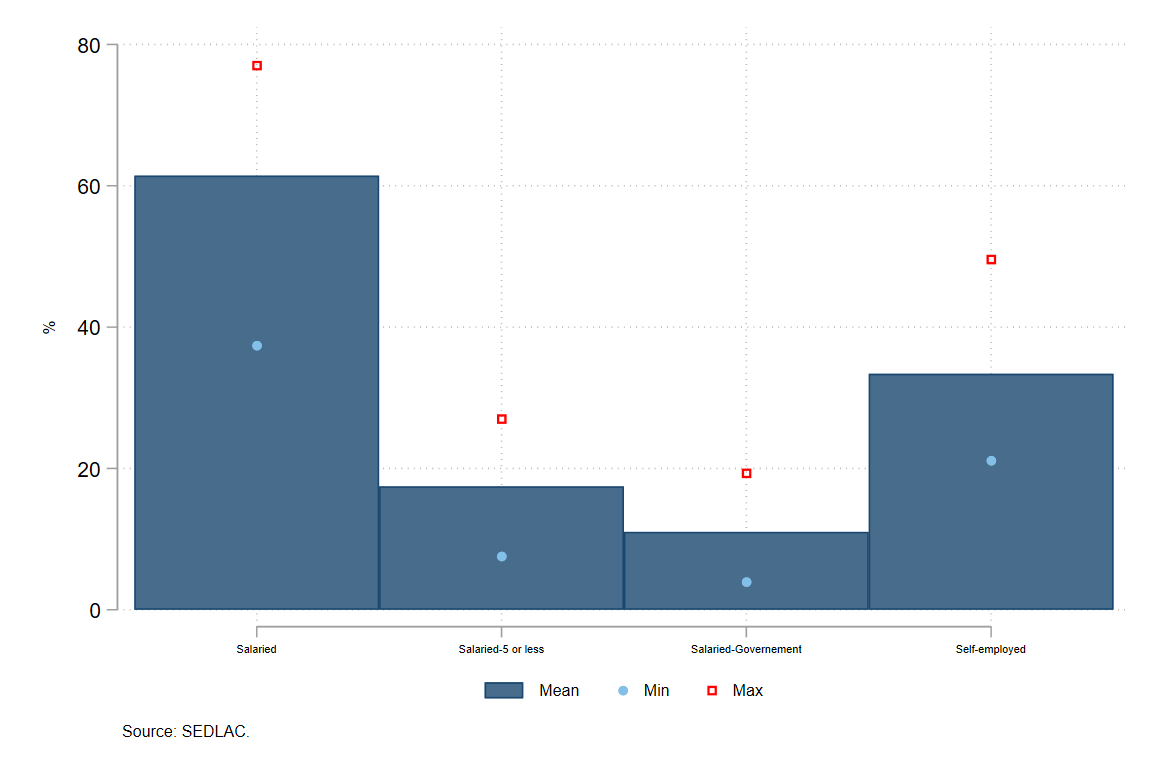
\includegraphics[scale=.3]{latex/figures/Snapshot/Structure of employment.png}
        \label{fig:employment}
        \footnotesize{Source: Household Surveys-SEDLAC.}
        \footnotesize{Note: Each bar is a simple average of country level weighted average in 2021. Countries included in the sample: Argentina, Bolivia, Brazil, Chile, Colombia, Costa Rica, Dominican Republic, Ecuador, El Salvador, Guatemala, Honduras, Mexico, Panama, Peru, Paraguay and Uruguay. Some countries don’t have information for 2021, in that cases we use the last available year, for Chile 2022, Guatemala 2014; Honduras 2019; Mexico 2018 and Uruguay 2019. The "non-salaried" category corresponds to unpaid workers such as family or cooperative workers.}
        \end{figure}

The structure of employment as depicted in the Figure \ref{fig:employment} reflects broader labor market dynamics characteristic of developing economies in Latin America, where informal and non-standard employment accounts for a significant portion of the workforce. The high level of self-employment and the existence of a substantial non-salaried sector point to the structural issues that perpetuate labor informality across the region.

Labor market segmentation, where a portion of the workforce is locked in low-productivity, informal sectors while a smaller, formal sector enjoys greater protections and higher wages, is a persistent issue in Latin America. The informal sector, typically composed of self-employed and non-salaried workers, tends to lack the social protections afforded to formal salaried workers. As De Soto’s (1989) classic work on the informal economy suggests, informal workers often operate outside of legal frameworks due to excessive regulatory burdens and limited access to formal employment opportunities.

In addition to De Soto’s perspective, the work of Perry et al. (2007) emphasizes the heterogeneity of informality, distinguishing between voluntary and involuntary informal workers. Many self-employed workers may opt for informal work due to greater flexibility or the inability to find formal jobs, while others are pushed into informality due to the lack of job opportunities in the formal sector. This duality is crucial for understanding the complexity of informality, as efforts to formalize employment should account for both sets of workers.

The Figure 3 provides a comparative analysis between salaried and self-employed workers across four key dimensions: education level, firm type, sector, and contributions to social security (SS). This section offers a concise academic analysis of each dimension, drawing on the information presented in the graph to highlight critical differences and inform broader discussions on labor market segmentation and informality.

\begin{figure}[h!tbp]
\centering
  \caption{Structure of salaried and self-employed workers}
  \subcaption{\textbf{Education level}}
    \begin{subfigure}{.5\textwidth}
  \centering
    \footnotesize{$Salaried$}
  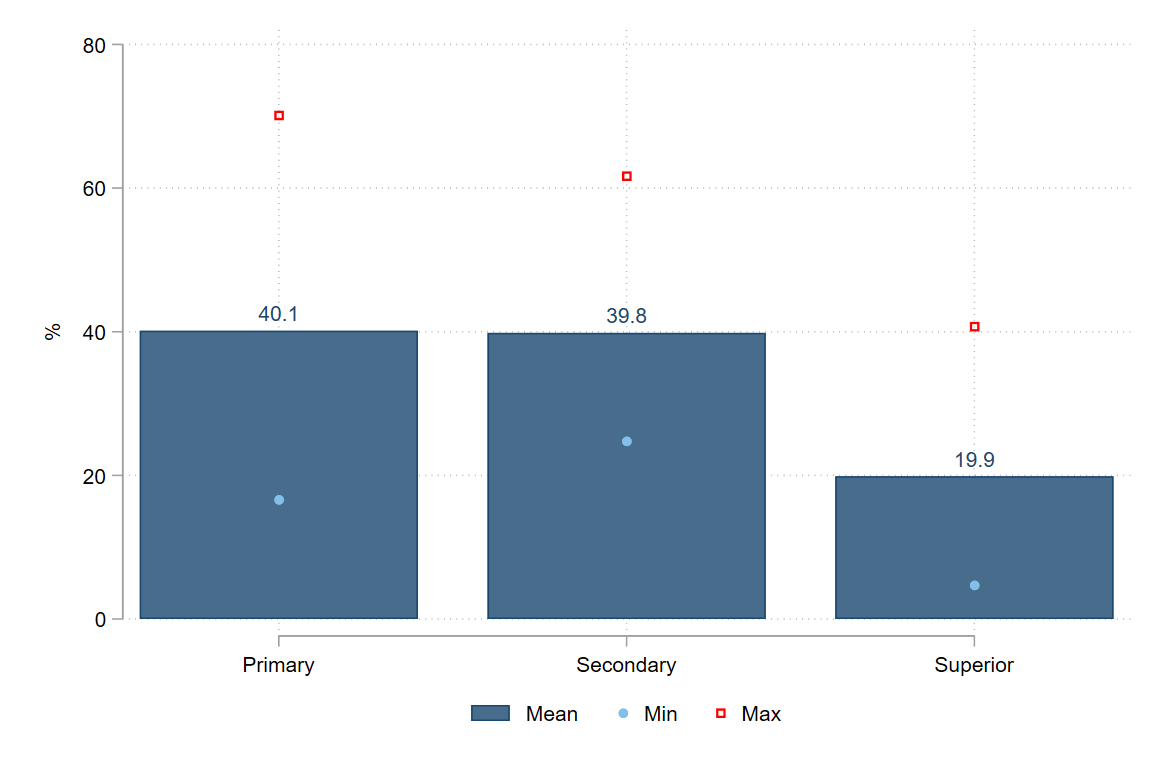
\includegraphics[width=1\textwidth]{latex/figures/Snapshot/Salaried-education.png}
  \label{fig:salariededuc}
\end{subfigure}%
\begin{subfigure}{.5\textwidth}
  \centering
    \footnotesize{$Self employed$}
  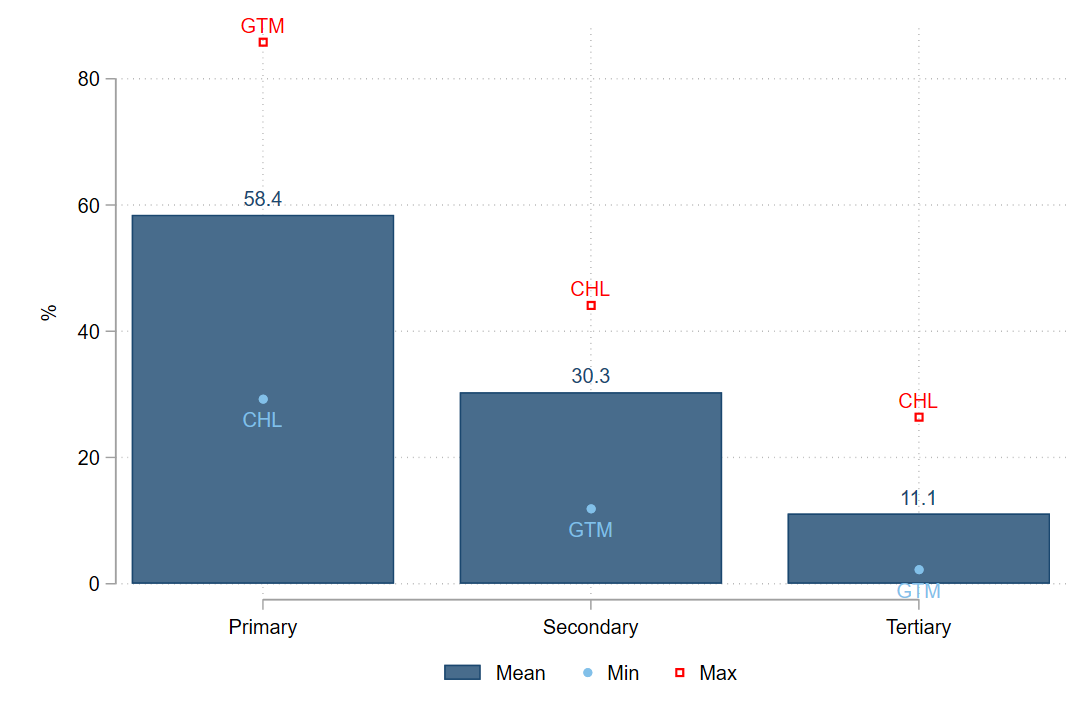
\includegraphics[width=1\textwidth]{latex/figures/Snapshot/Self employed-education.png}
  \label{fig:selfeduc}
\end{subfigure}

\subcaption{\textbf{Firm type}}
\begin{subfigure}{.5\textwidth}
  \centering
    \footnotesize{$Salaried$}
  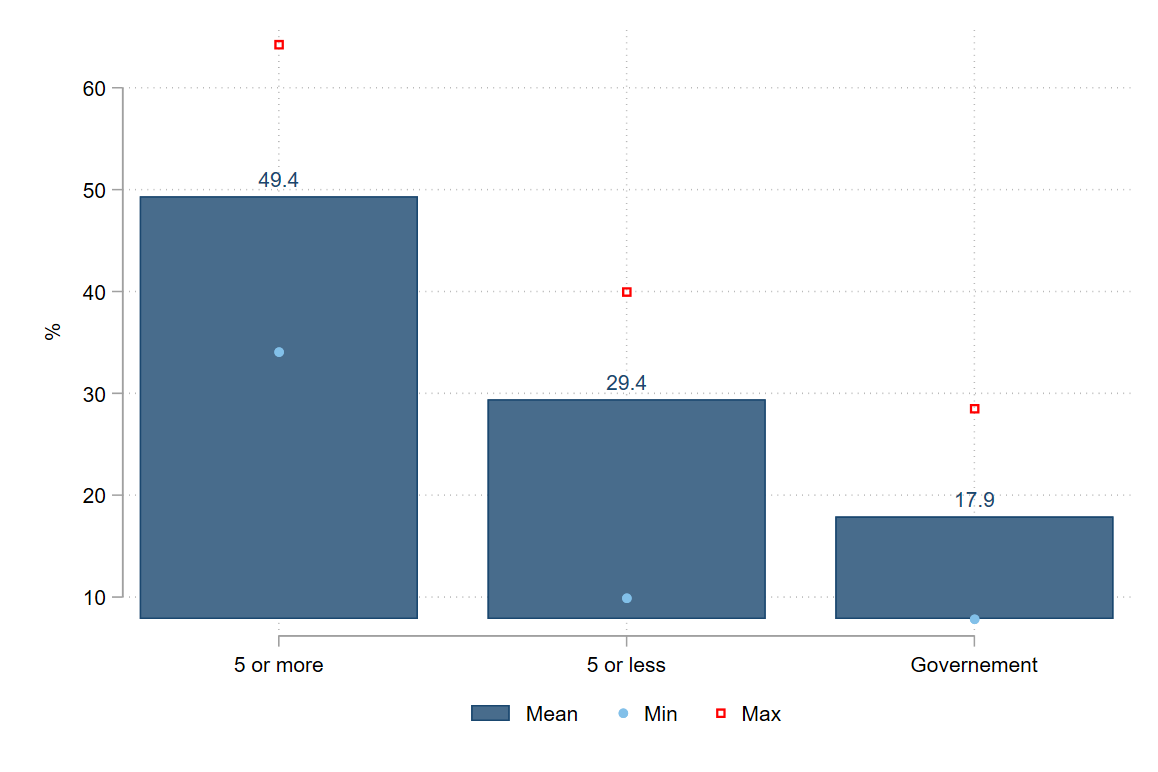
\includegraphics[width=1\textwidth]{latex/figures/Snapshot/Salaried-firmsize.png}
  \label{fig:salariedfirmsize}
\end{subfigure}%
\begin{subfigure}{.5\textwidth}
  \centering
    \footnotesize{$Self employed$}
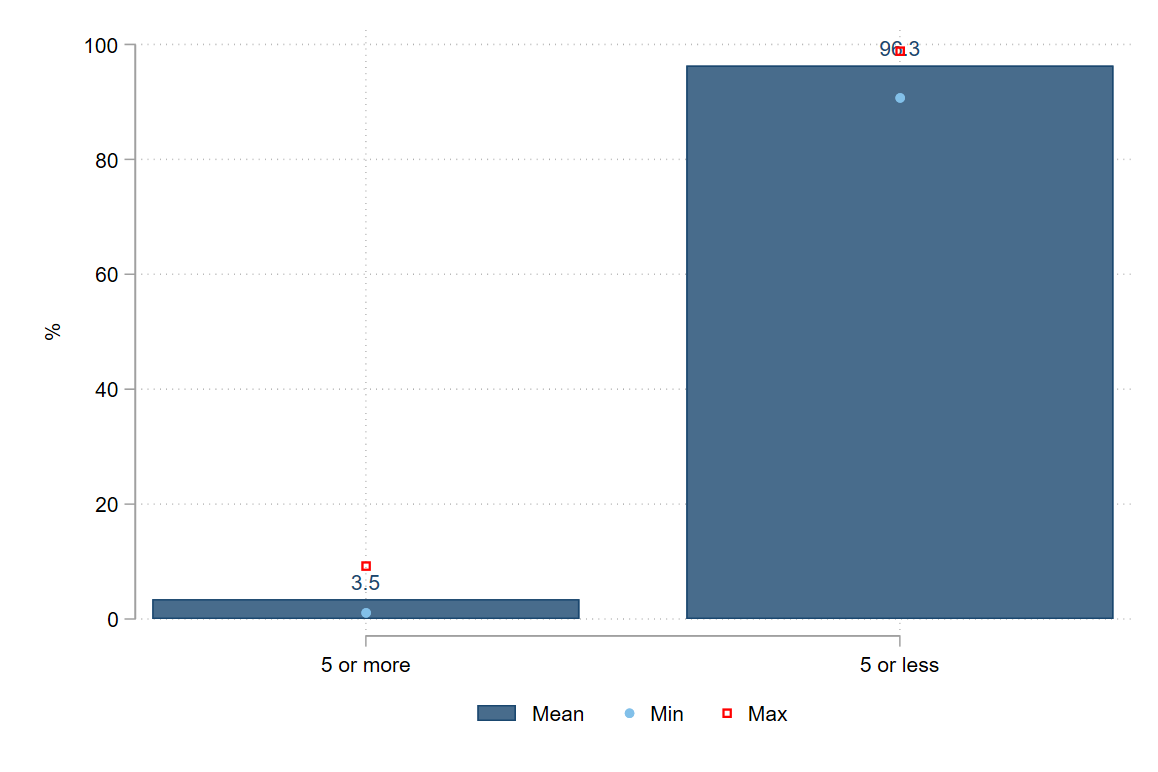
\includegraphics[width=1\textwidth]{latex/figures/Snapshot/Self employed-firmsize.png}
  \label{fig:selfirmsize}
\end{subfigure}

\subcaption{\textbf{Sector}}
\begin{subfigure}{.5\textwidth}
  \centering
  \footnotesize{$Salaried$}
  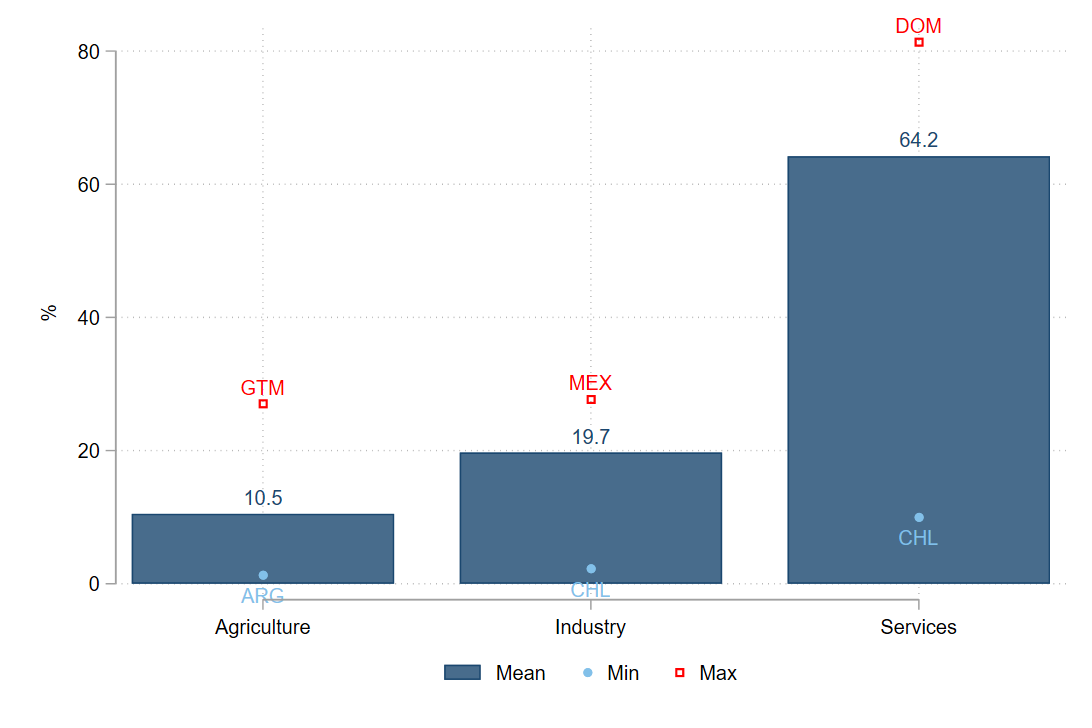
\includegraphics[width=1\textwidth]{latex/figures/Snapshot/Salaried-sector.png}
  \label{fig:salariedsector}
\end{subfigure}%
\begin{subfigure}{.5\textwidth}
  \centering
  \footnotesize{$Self employed$}
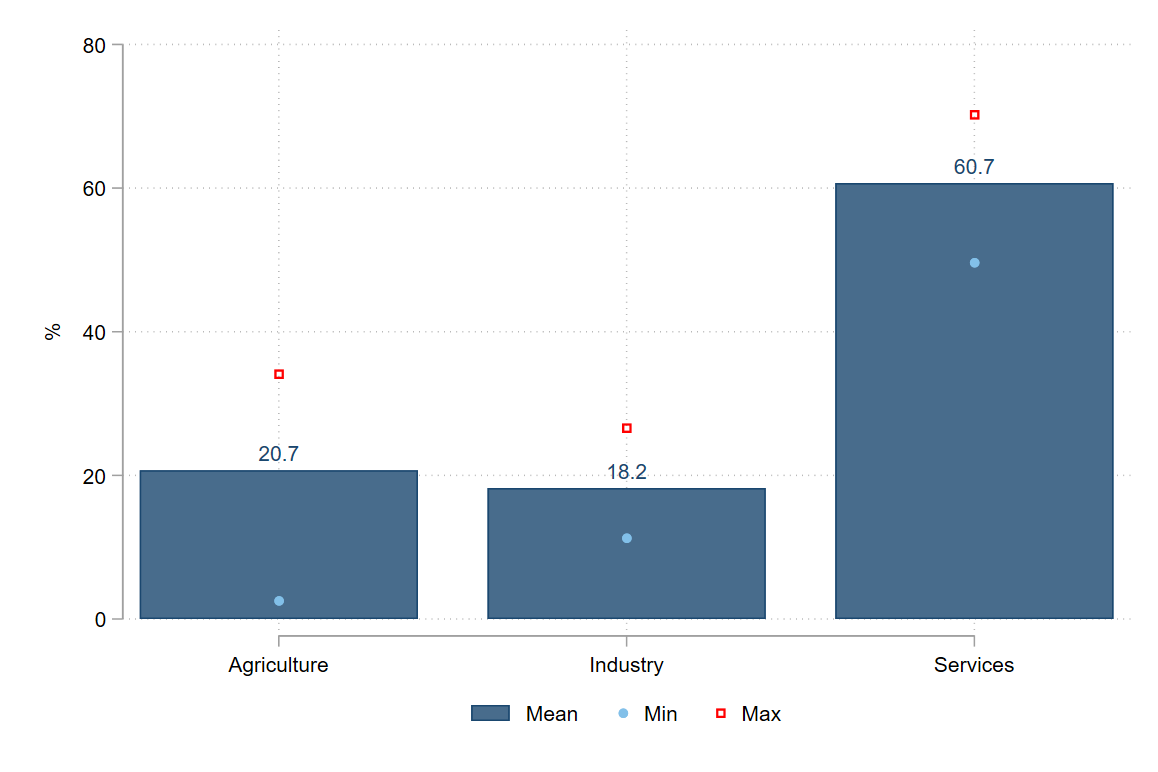
\includegraphics[width=1\textwidth]{latex/figures/Snapshot/Self employed-sector.png}
  \label{fig:selfsector}
\end{subfigure}

\subcaption{\textbf{Contributions to SS}}
\begin{subfigure}{.5\textwidth}
  \centering
    \footnotesize{$Salaried$}
  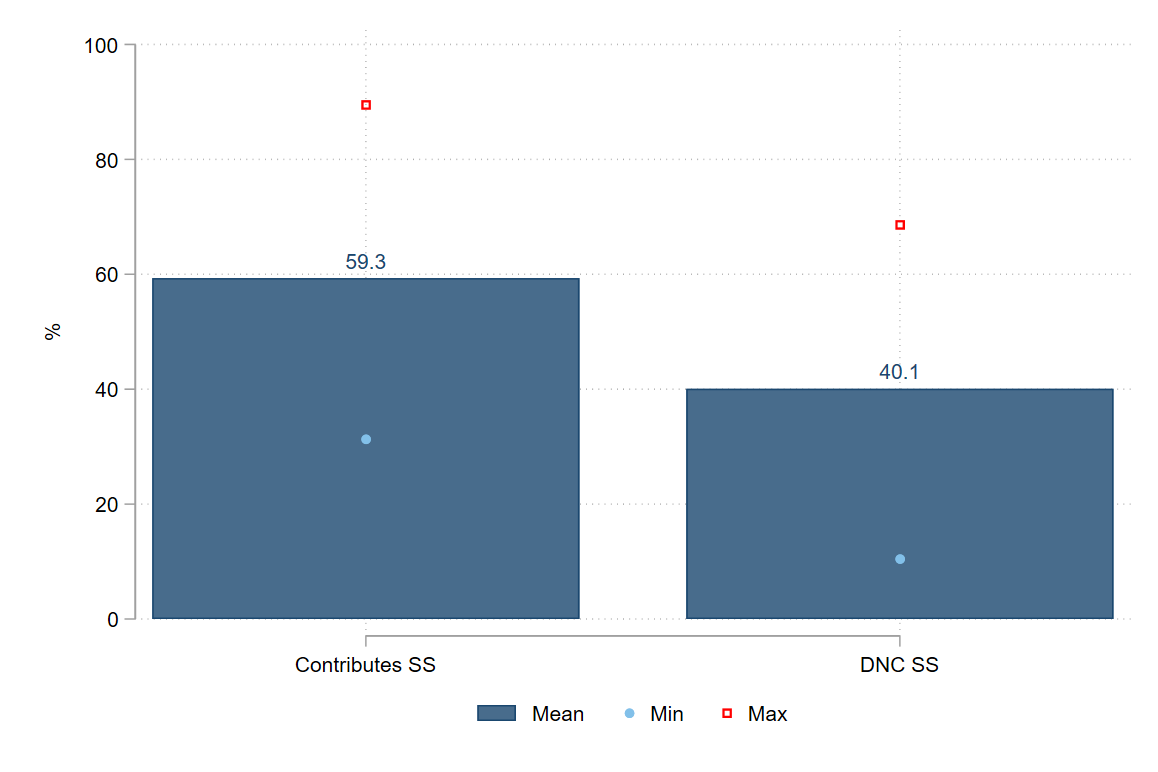
\includegraphics[width=1\textwidth]{latex/figures/Snapshot/Salaried-SS.png}
  \label{fig:salariedSS}
\end{subfigure}%
\begin{subfigure}{.5\textwidth}
  \centering
\footnotesize{$Self employed$}
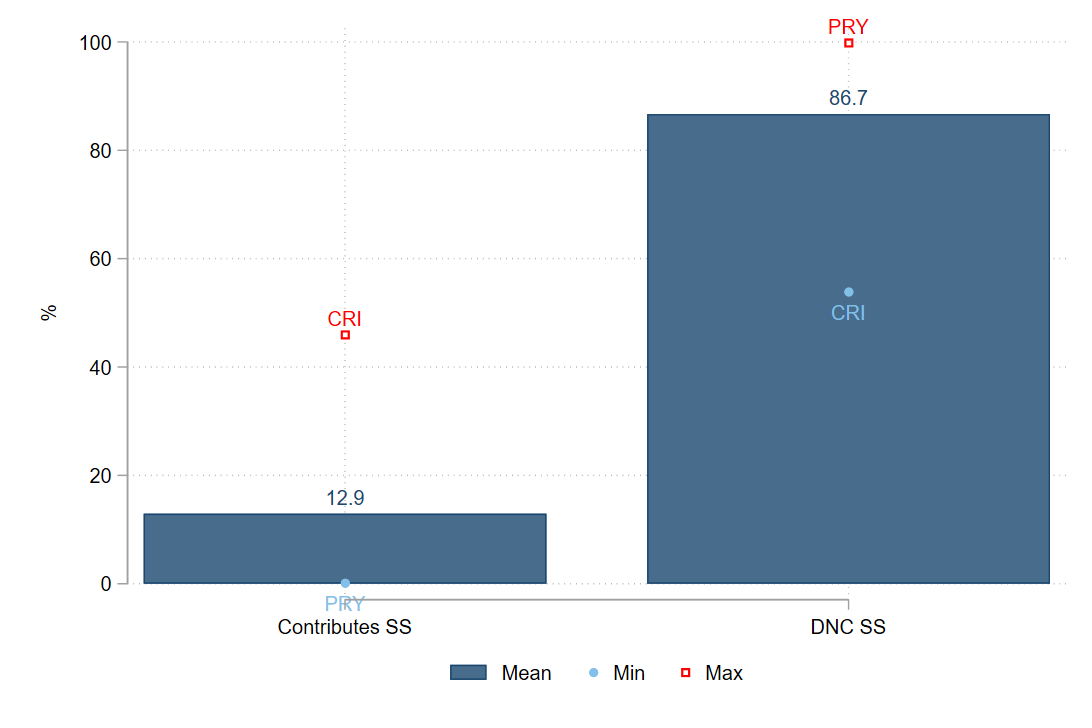
\includegraphics[width=1\textwidth]{latex/figures/Snapshot/Self employed-SS.png}
  \label{fig:selfSS}
\end{subfigure}
\justifying
\footnotesize{Source: Household Surveys-SEDLAC.}
\footnotesize{Note: Each bar is a simple average of country level weighted average in 2021. Countries included in the sample: Argentina, Bolivia, Brazil, Chile, Colombia, Costa Rica, Dominican Republic, Ecuador, El Salvador, Guatemala, Honduras, Mexico, Panama, Peru, Paraguay and Uruguay. Some countries don’t have information for 2021, in that cases we use the last available year, for Chile 2022, Guatemala 2014; Honduras 2019; Mexico 2018 and Uruguay 2019. Argentina and Chile are excluded from contributions to Social security of self-employed figure, because this question is available only for salaried workers. Also, Chile is excluded from calculations of self-employed in sectors, because is only for salaried workers.}

\end{figure}

\begin{enumerate}
\item Education Level

The distribution by education level shows that the majority of salaried workers have a secondary education (39.8\%), while a smaller portion has tertiary education (19.9\%). This suggests that formal employment opportunities increase with higher levels of education, consistent with human capital theory, which emphasizes the role of education in accessing formal, higher-paying jobs. In contrast, a large proportion of self-employed workers have only a primary education (53.4\%), with very few holding tertiary degrees (11.1\%). This indicates that self-employment is often a fallback for workers with lower educational attainment, which correlates with informality and lower productivity.

\item Firm Type

Nearly half of salaried workers are employed in firms with 5 or more employees (49.4\%), which suggests a formalized, structured employment environment. A notable share also works in government positions (17.9\%), highlighting the role of the public sector in offering formal employment. The majority of self-employed workers operate in firms with 5 or fewer employees (96.3\%), indicating the small-scale, often informal nature of their work. The minimal presence of self-employed workers in larger firms reflects the challenges in scaling self-employment into more formal, larger enterprises.

\item Sector

A significant portion of salaried workers is concentrated in the services sector (64.2\%), reflecting the growing importance of service-oriented industries in formal employment. Industry (19.7\%) and agriculture (10.5\%) represent smaller shares, with salaried jobs likely tied to higher productivity activities in these sectors. Self-employed workers are also heavily concentrated in the services sector (60.7\%), though their participation in agriculture (29.7\%) is notably higher than salaried workers, suggesting a strong link between agricultural self-employment and informal labor.

\item Contributions to Social Security (SS)

The majority of salaried workers (59.3\%) contribute to social security, underscoring the formalized nature of their employment. However, a substantial minority (40.1\%) does not contribute, highlighting ongoing challenges in ensuring universal coverage, even within formal employment categories. In stark contrast, only 12.9\% of self-employed workers contribute to social security, signaling the high level of informality and lack of social protection among this group. This reflects the broader issue of exclusion from social safety nets for informal and self-employed workers, contributing to their economic vulnerability.
\end{enumerate}

The graph provides a clear depiction of the segmentation in labor markets between salaried and self-employed workers. Salaried workers are more likely to have higher education, work in larger firms, be employed in services, and contribute to social security—features typically associated with formality. Conversely, self-employed workers tend to have lower educational attainment, work in small or informal settings, engage in agriculture, and lack social protection. These disparities highlight the challenges of informality in Latin American labor markets and underscore the need for policies aimed at improving education, formalization of self-employment, and expanding social security coverage to informal workers.


Also, the Figure \ref{fig:employmentbars} presents a clearer evidence of the segmentation between salaried and self-employed workers, where salaried workers are more likely to be found in formal, larger firms and are better represented in social security systems. Meanwhile, self-employed workers tend to have lower educational attainment, work in small-scale firms, and are concentrated in sectors associated with high informality. This structural divide underscores the challenges of labor informality in Latin America, particularly in addressing the social vulnerability of self-employed workers who lack education and access to formal protections. Strategies aimed at enhancing formalization, particularly for the self-employed and low-skilled workers, are essential for creating more inclusive labor markets.

\begin{figure}[h!tbp]
        \centering
        \caption{Structure of employment salaried and self-employed workers}     
        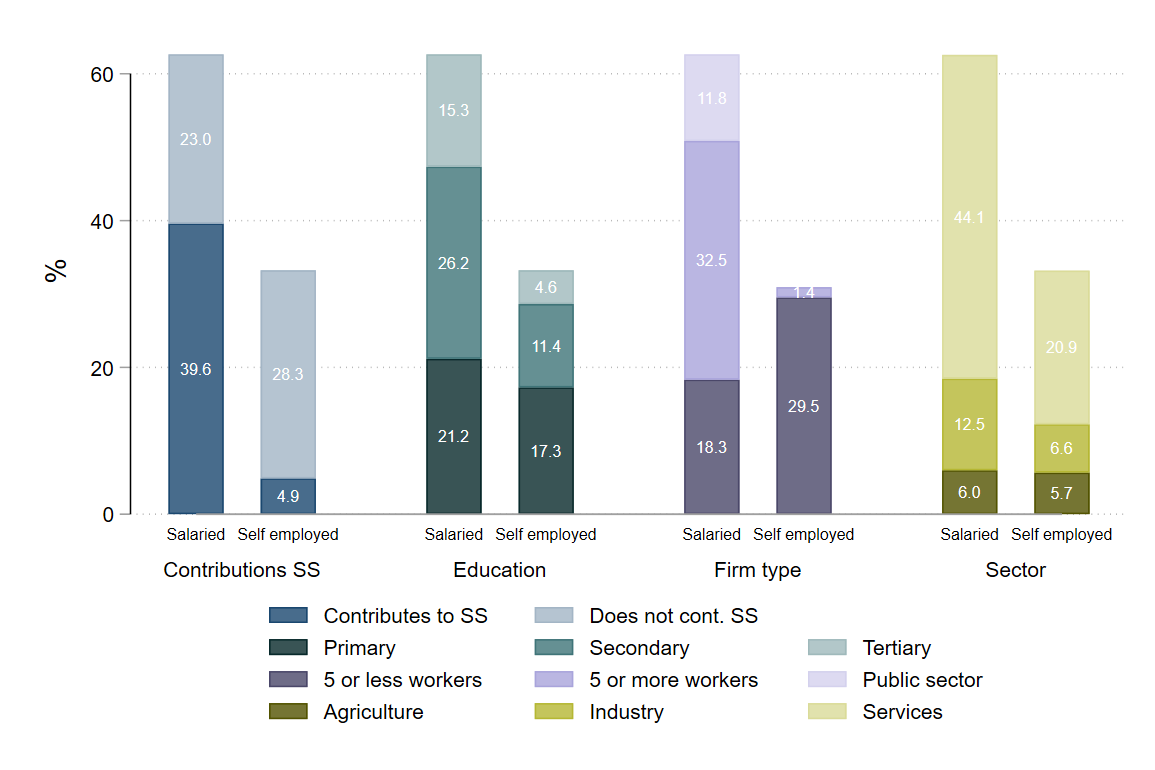
\includegraphics[scale=.3]{latex/figures/Snapshot/Snapshot salaried and self-employed.png}
        \label{fig:employmentbars}
\justifying
\footnotesize{Source: Household Surveys-SEDLAC.}
\footnotesize{Note: Each bar is a simple average of country level weighted average in 2021. Countries included in the sample: Argentina, Bolivia, Brazil, Chile, Colombia, Costa Rica, Dominican Republic, Ecuador, El Salvador, Guatemala, Honduras, Mexico, Panama, Peru, Paraguay and Uruguay. Some countries don’t have information for 2021, in that cases we use the last available year, for Chile 2022, Guatemala 2014; Honduras 2019; Mexico 2018 and Uruguay 2019. Argentina and Chile are excluded from contributions to Social security of self-employed graph, because this question is available only for salaried workers. Also, Chile is excluded from calculations of self-employed in sectors, because is only for salaried workers.}

\end{figure}

\begin{enumerate}

\item Contributions to Social Security (SS)

A significant proportion (38.5\%) contribute to social security, showing a relatively high level of formality in employment. However, 24.6\% of salaried workers do not contribute, signaling a portion of the formal sector that remains outside the social protection system. A striking 25.3\% of the self-employed do not contribute to social security, while only 3.8\% are part of the system. This indicates a much higher rate of informality among the self-employed, as the majority are excluded from social protection mechanisms.

\item Education

The education levels of salaried workers are more evenly distributed across categories, with 24.7\% having completed primary education (C1), 24.5\% having completed secondary education (C2), and 10.1\% possessing higher education (C3). This suggests that formal salaried employment is accessible at varying education levels, though more formal positions tend to require secondary or tertiary education. In contrast, the self-employed are heavily concentrated in lower education categories, with 19.5\% having only primary education and just 3.7\% completing tertiary education. This confirms the link between lower education levels and self-employment, often associated with informal sectors.

\item Firm Type

The majority of salaried workers are employed in larger firms (C2, with 49.4\% in firms with more than 5 employees) and the public sector (C3, 16.1\%). Smaller firms (C1, 29.4\%) still represent a significant portion but are less dominant. Unsurprisingly, 98.3\% of self-employed workers operate in very small firms with five or fewer employees (C1), illustrating the small-scale nature of most self-employment and reinforcing the connection to informality.

\item Sector

Most salaried workers are concentrated in the services sector (C3, 39.4\%), which is typical for formal employment. Meanwhile, 6.4\% are in agriculture (C1), and 12.1\% are in industry (C2), highlighting the concentration of salaried employment in services. The self-employed exhibit a similar pattern, with 19.0\% in services, but a larger share (6.5\%) are engaged in agriculture, reflecting the prevalence of informal agricultural work.

   \end{enumerate}

        
\item Structure of Employment II - Sector and Contribution to SS

\begin{figure}[h!tbp]
        \justifying
        \caption{Structure of employment by sector}     
        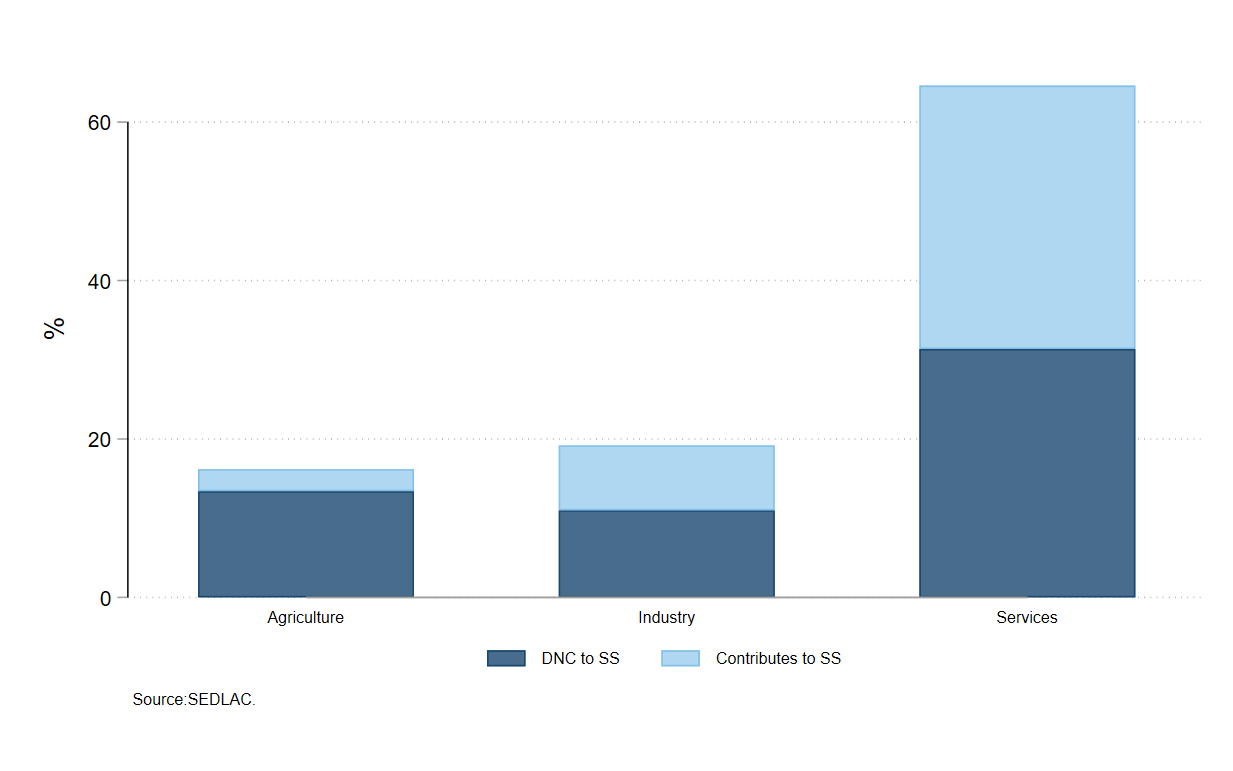
\includegraphics[scale=.3]{latex/figures/Snapshot/Structure of employment and sector.png}
        \label{fig:sector}
       \footnotesize{Source: Household Surveys-SEDLAC.}
        \footnotesize{Note: Each bar is a simple average of country level weighted average in 2021. Countries included in the sample: Bolivia, Brazil, Chile, Colombia, Costa Rica, Dominican Republic, Ecuador, El Salvador, Guatemala, Honduras, Mexico, Panama, Peru, Paraguay and Uruguay. Some countries don’t have information for 2021, in that cases we use the last available year, for Chile 2022, Guatemala 2014; Honduras 2019; Mexico 2018 and Uruguay 2019. Argentina is excluded from this figure because the household survey is urban.}
\end{figure}

        
\item Employment by Firm Size
\begin{figure}[h!tbp]
        \justifying
        \caption{Structure of private employment by firm size}     
        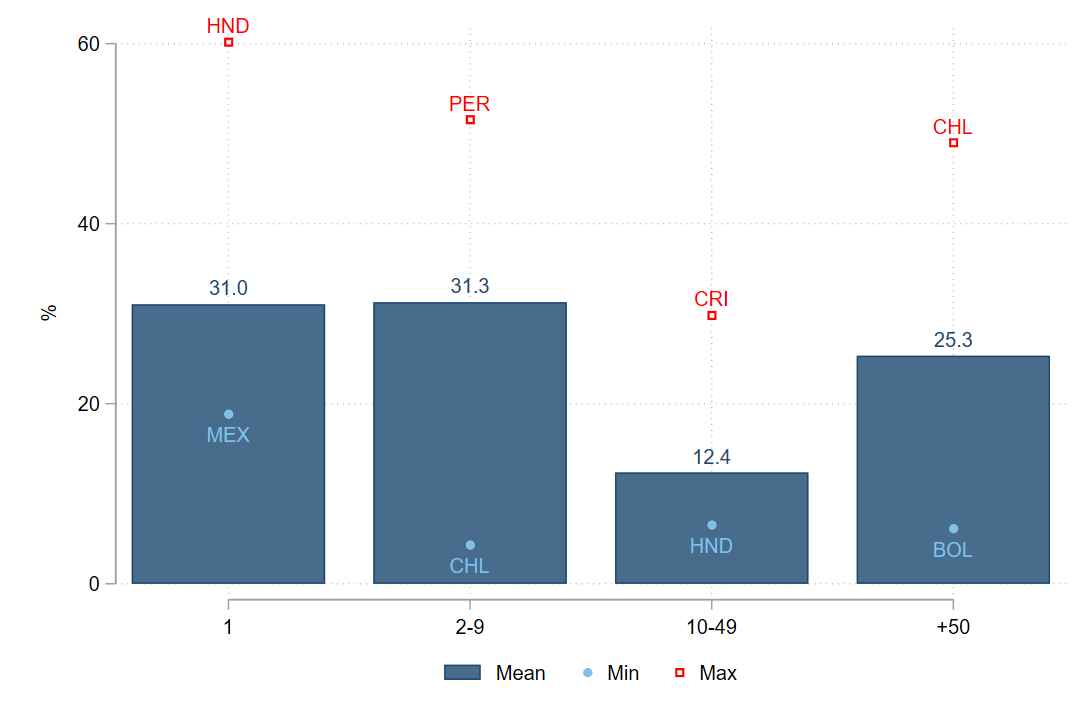
\includegraphics[scale=.3]{latex/figures/Snapshot/Structure of employment by firm size.png}
        \label{fig:firmsize}
        \footnotesize{Source: Household Surveys-SEDLAC.}
        \footnotesize{Note: Each bar is a simple average of country level weighted average in 2021. Countries included in the sample: Bolivia, Brazil, Chile, Colombia, Costa Rica, Ecuador, El Salvador, Honduras, Mexico, Panama, Peru, Paraguay and Uruguay. Some countries don’t have information for 2021, in that cases we use the last available year, for Chile 2022, Guatemala 2014; Honduras 2019; Mexico 2018 and Uruguay 2019. We exclude Argentina, Dominican Republic and Guatemala, because of missing information in firm size variable.}
        \end{figure}


        
 \item Social security contributions

        \begin{figure}[h!tbp]
        \justifying
        \caption{Share of Workers Who Do Not Contribute to Social Security by Selected Characteristics}     
        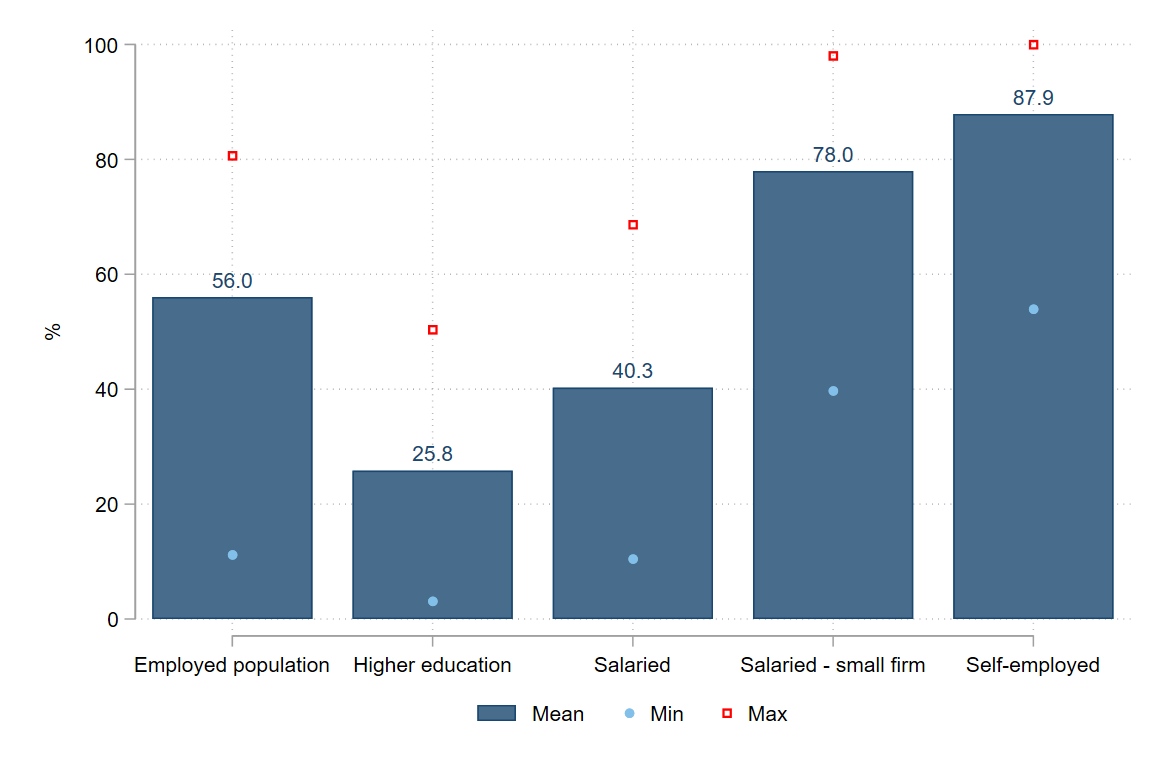
\includegraphics[scale=.3]{latex/figures/Snapshot/Social security contributions.png}
        \label{fig:SScontributions}
        \footnotesize{Source: Household Surveys-SEDLAC.}
        \footnotesize{Note: Each bar is a simple average of country level weighted average in 2021. Countries included in the sample: Argentina, Bolivia, Brazil, Chile, Colombia, Costa Rica, Dominican Republic, Ecuador, El Salvador, Guatemala, Honduras, Mexico, Panama, Peru, Paraguay and Uruguay. Some countries don’t have information for 2021, in that cases we use the last available year, for Chile 2022, Guatemala 2014; Honduras 2019; Mexico 2018 and Uruguay 2019. \textbf{The groups are not exclusive.} "Tertiary education" corresponds to people in the workforce who have completed tertiary level of education. "Salaried-Small firm" are salaried employees that work in a firm of 5 or less workers.}
        \end{figure}


\item Life cycle- self employment and salaried informal
 \begin{figure}[h!tbp]
        \justifying
        \caption{Average Age profile in a LAC country}     
        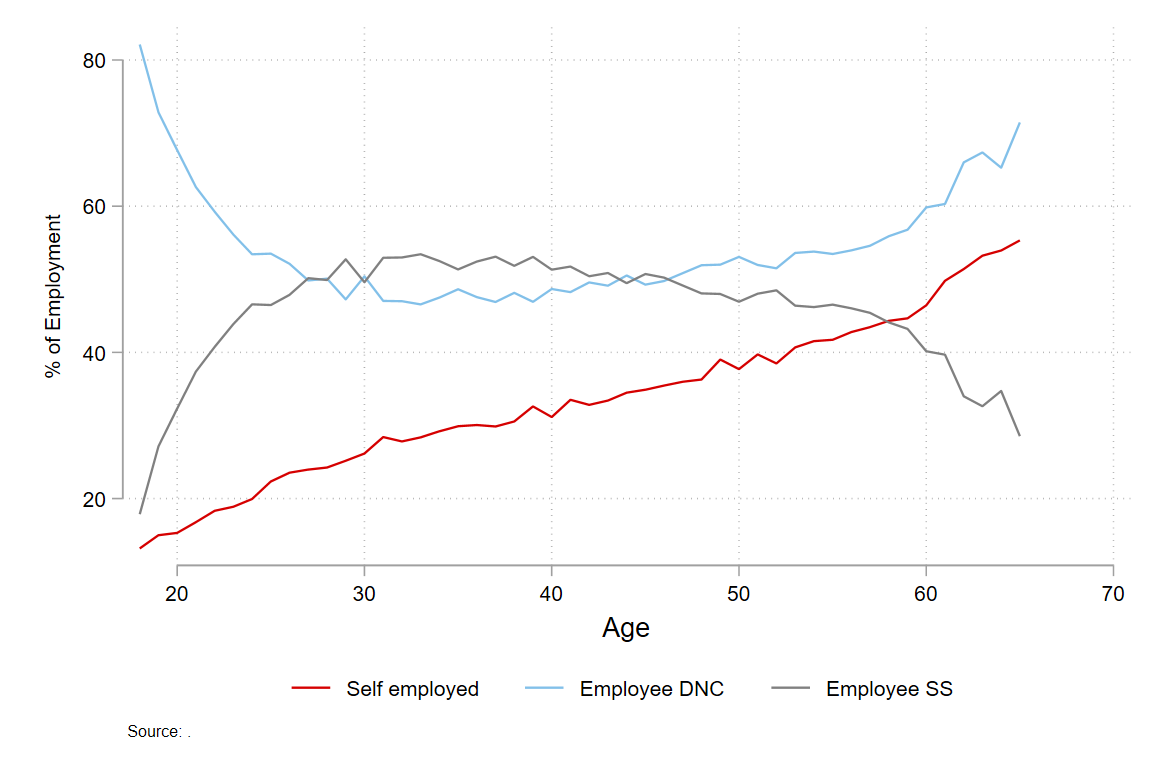
\includegraphics[scale=.3]{latex/figures/Snapshot/age_profile.png}
        \label{fig:age_pro}
        \footnotesize{Source: Household Surveys-SEDLAC.}
        \footnotesize{Note: Each line is a simple average of country level data. Country level data is computed weighting by total workers. Countries included in the sample: Argentina, Bolivia, Brazil, Chile, Colombia, Costa Rica, Dominican Republic, Ecuador, El Salvador, Guatemala, Honduras, Mexico, Panama, Peru, Paraguay and Uruguay. Data corresponds to 2021 except for  Chile (2022), Guatemala (2014); Honduras (2019); Mexico (2018) and Uruguay (2019).}
        \end{figure}
\item Decomposition of changes in the informality rate

\end{enumerate}
   
     
\section{Dynamics: last 20 years}  

\subsection{Cross country figures}
\subsubsection{Household}

\begin{figure}[h!tbp]
    \justifying
     \caption{Snapshot of LAC’s household contribution status}     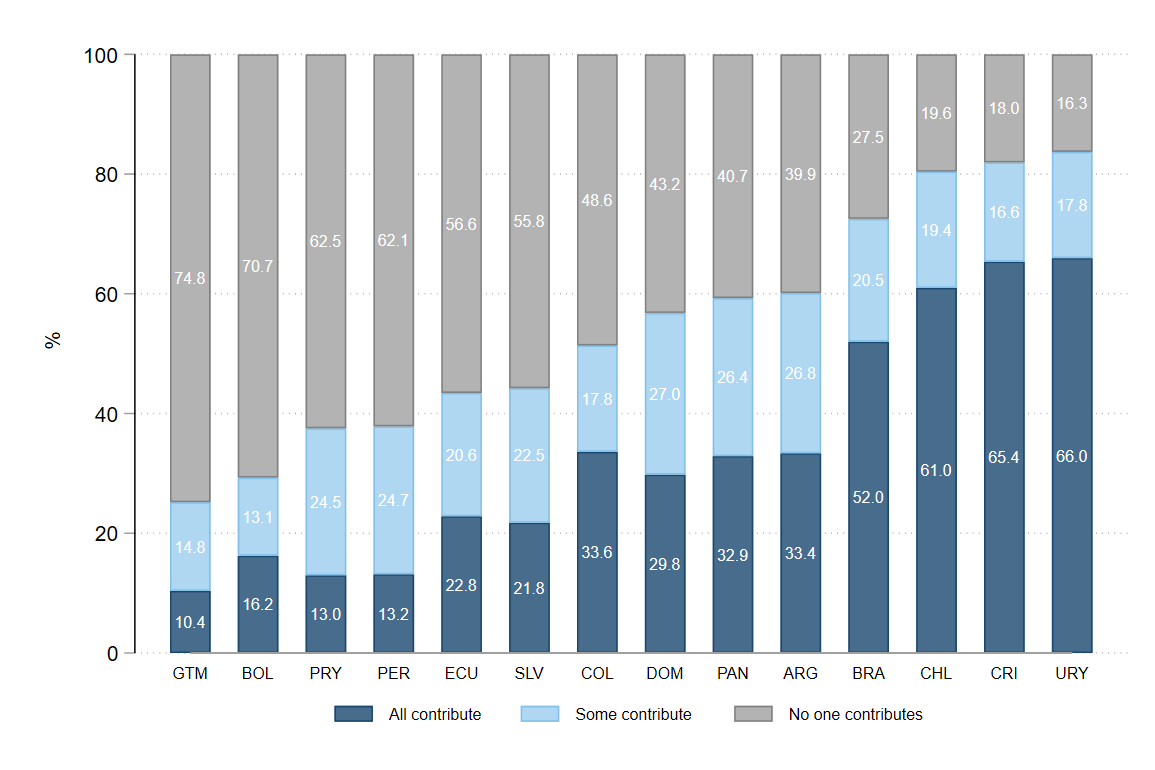
\includegraphics[scale=.3]{latex/figures/Household/snapshot_household.png}
    \label{fig:Householdlastyear}
    \footnotesize{Source: Household Surveys-SEDLAC.}
    \footnotesize{Note: Each bar is a weighted average of each country, weighting by total workers in 2021. Data corresponds to 2021 except for Chile 2022, Guatemala 2014; Honduras 2019; Mexico 2018 and Uruguay 2019.}
    \footnotesize{Note: The figure reports the household contribution status to social security of households with at least one member works.   All contribute: corresponds to the percentage of households where all workers contribute to SS. Some contribute: corresponds to the percentage of households where some workers contribute to SS but not all. DNC – has partner: corresponds to the percentage of households where any worker contributes to SS, but the head of household have a partner. DNC – no partner: corresponds to the percentage of households where any worker contributes to SS, but the head of household do not have a partner.}
\end{figure}

\subsubsection{Individual level} %De este nombre no estoy segura

\begin{figure}[h!tbp]
    \justifying
     \caption{Employees who do not contribute to SS}     
     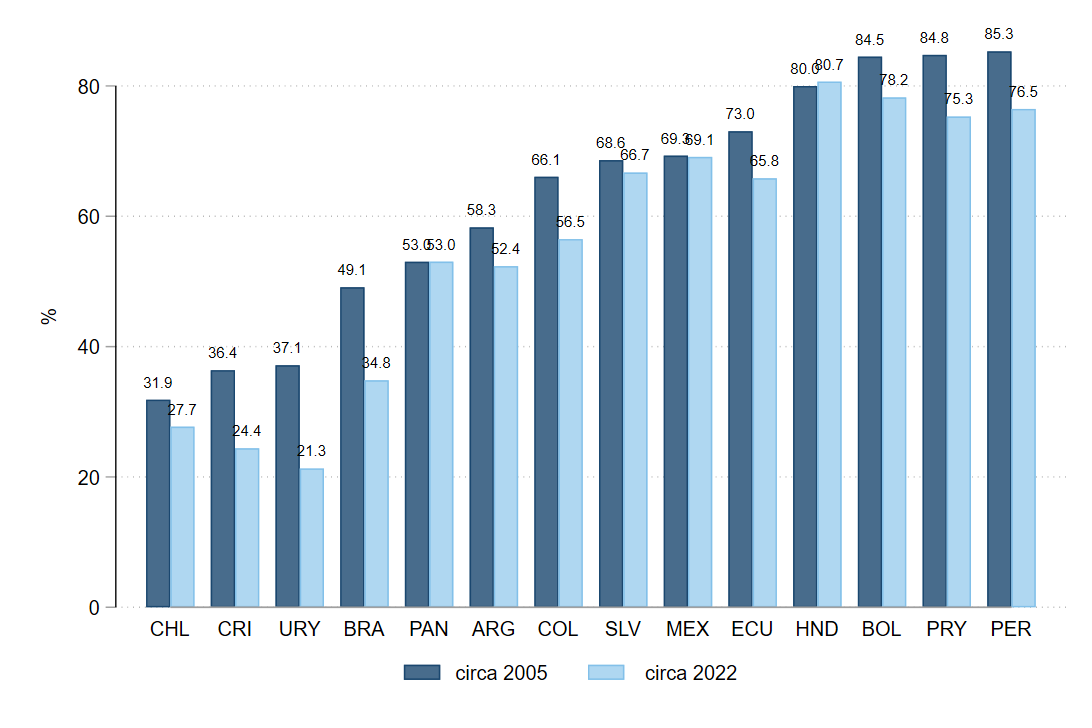
\includegraphics[scale=.3]{latex/figures/Snapshot/snapshot_informal_ss.png}
    \label{fig:SalariedSS}
    \footnotesize{Source: Household Surveys-SEDLAC.}
    \footnotesize{Note: Each bar is a weighted average of each country, weighting by total workers in 2005 and 2021.  Data corresponds to 2021 except for Chile 2022, Guatemala 2014; Honduras 2019; Mexico 2018 and Uruguay 2019.}
\end{figure}

\begin{figure}[h!tbp]
    \justifying
     \caption{Salaried who do not contribute to SS}     
     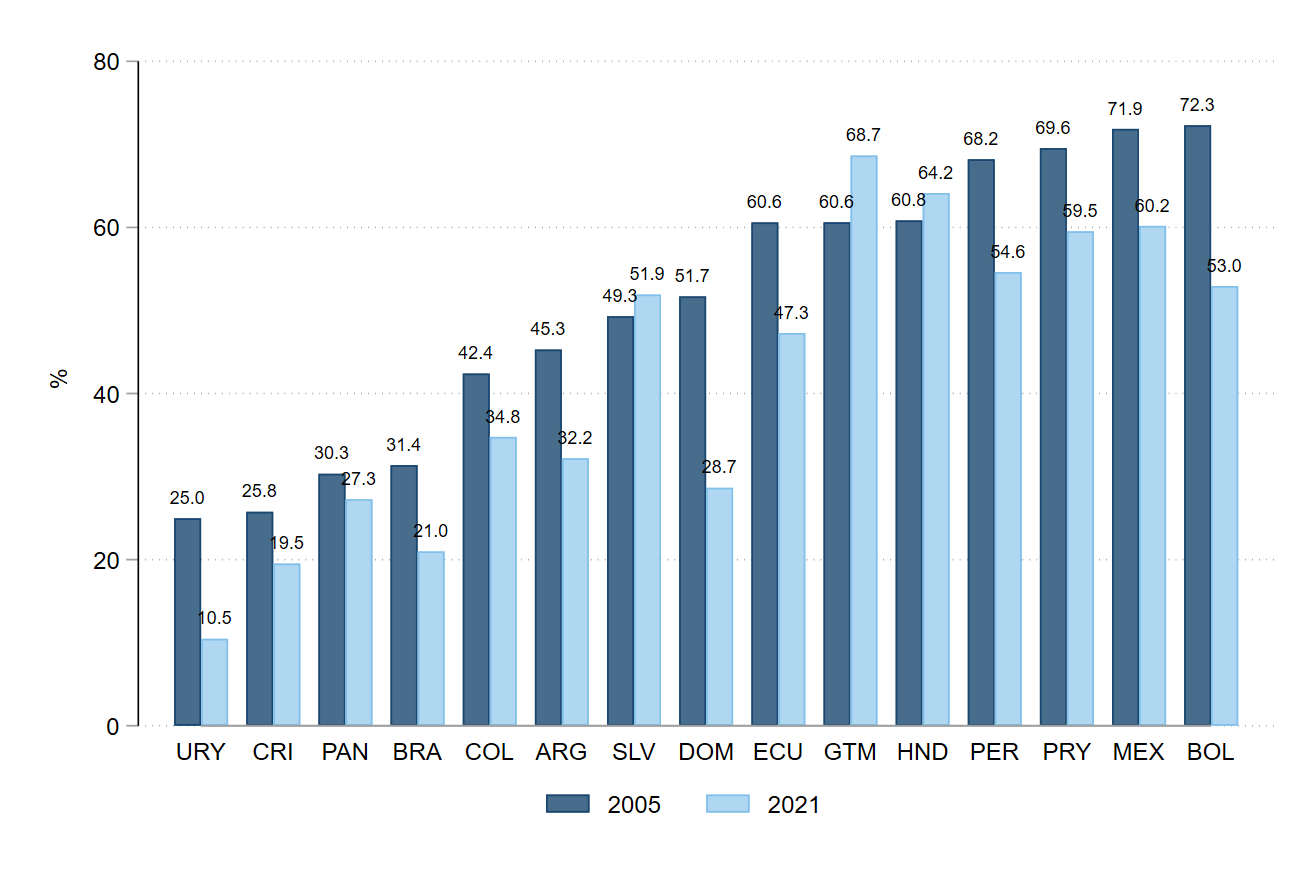
\includegraphics[scale=.3]{latex/figures/Snapshot/snapshot_informal_ss_dep.png}
    \label{fig:SalariedSS}
    \footnotesize{Source: Household Surveys-SEDLAC.}
    \footnotesize{Note: Each bar is a weighted average of each country, weighting by total workers in 2005 and 2021.  Data corresponds to 2021 except for Chile 2022, Guatemala 2014; Honduras 2019; Mexico 2018 and Uruguay 2019.}
\end{figure}

\begin{figure}[h!tbp]
    \justifying
     \caption{Salaried who work at small firms}     
     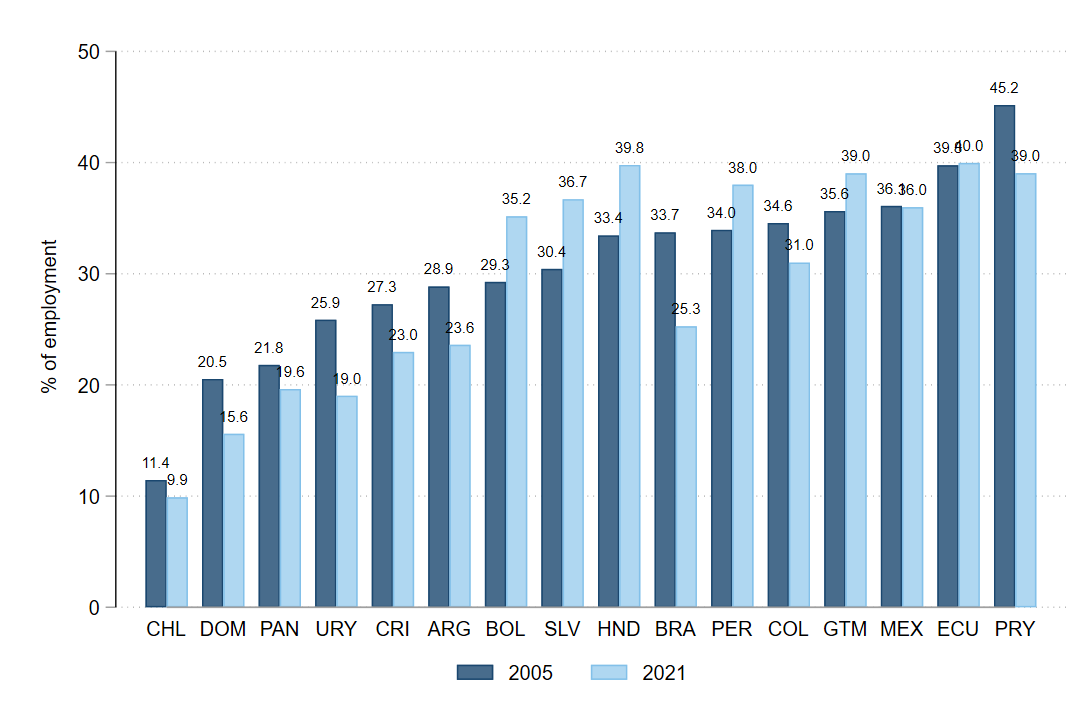
\includegraphics[scale=.3]{latex/figures/Snapshot/snapshot_dependents_small.png}
    \label{fig:SalariedSmall}
    \footnotesize{Source: Household Surveys-SEDLAC.}
    \footnotesize{Note: Each bar is a weighted average of each country, weighting by total workers in 2005 and 2021.  Data corresponds to 2021 except for Chile 2022, Guatemala 2014; Honduras 2019; Mexico 2018 and Uruguay 2019.}
\end{figure}

      

\begin{figure}[h!tbp]
        \justifying
        \caption{Microeconometric decomposition of evolution of workers who does not contribute to ss 2005-2021}     
        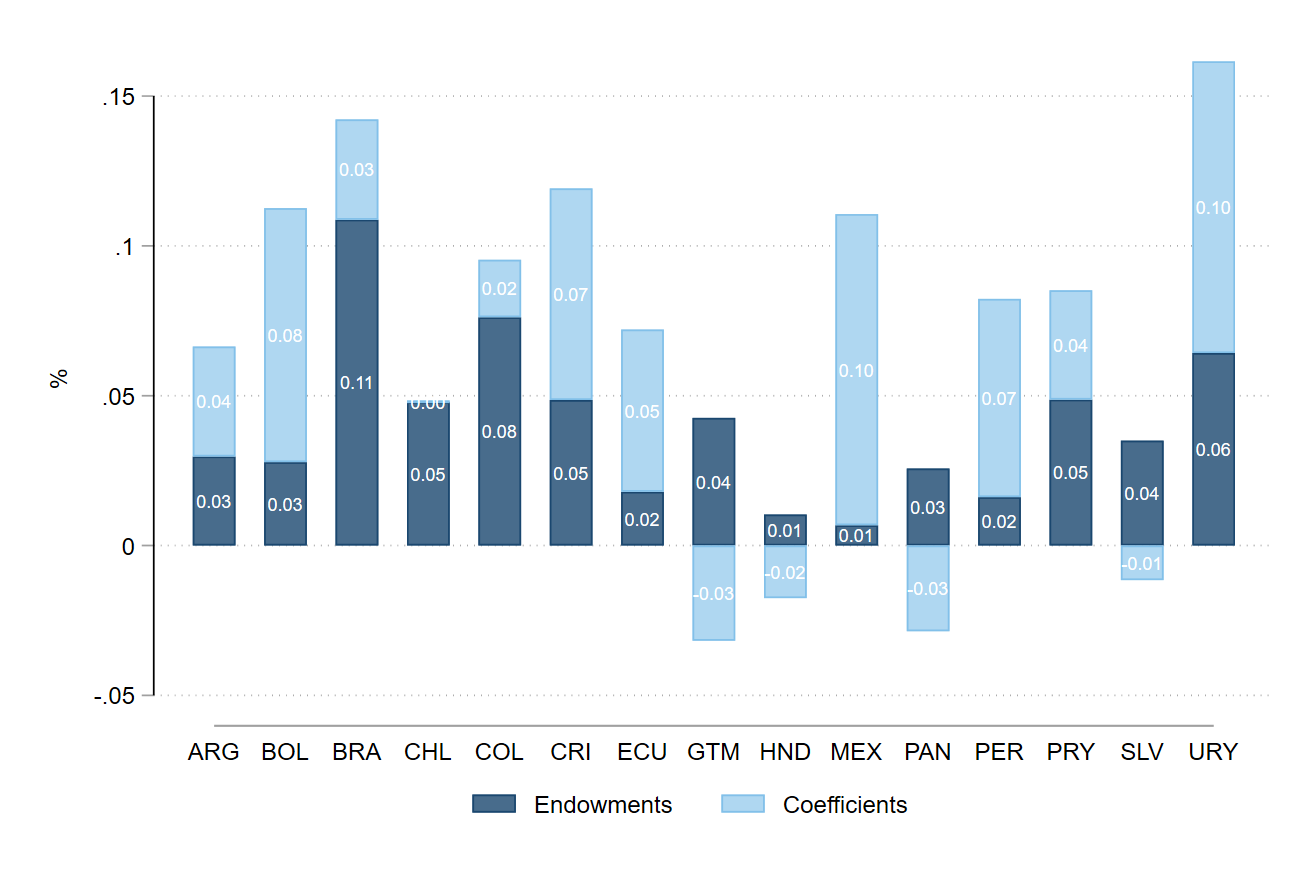
\includegraphics[scale=.3]{latex/figures/Snapshot/Oaxaca decomposition level.png}
        \label{fig:Oaxaca_level}
        \footnotesize{Source: Household Surveys-SEDLAC.}
        \footnotesize{Note: Each bar is the actual change in Social security contributions corresponds to the level of coefficients and the level of the endowment effects.  Data corresponds to 2021 except for Chile 2022, Guatemala 2014; Honduras 2019; Mexico 2018 and Uruguay 2019.}
        \end{figure}

\section{Appendix}
\subsection{Oaxaca methodology decomposition}
In order to determine the extent to which the change in the formality rate among wage earners in each country being studied is due to variations in the composition of employment (composition effect) and to what extent it is due to the formality rate of each group of workers (coefficient effect), an "aggregate" decomposition was calculated as a first step, as follows:

${\Delta}LF=\sum_{g=1}^{G}w_g^{0}.{\Delta}LF_g+\sum_{g=1}^{G}LF_g^{0}.{\Delta}w_g$

where:
\begin{itemize}

\item ${\Delta}LF$:change in labour formality rate between $t=1$ and $t=0$ 
\item ${\Delta}LF_g$:change in labour formality rate between $t=1$ and $t=0$ in subgroup g
\item ${\Delta}LF_g^{0}$:Labour formality rate of subgroup g in $t=0$
\item $w_g^{0}$:participation rate of group g in total wage earnerns in $t=0$
\item ${\Delta}w_g$:change in participation rate of group g in total wage earners between $t=1$ and $t=0$ 
\end{itemize}

The first term in the equation reflects the coefficient effect, which is the weighted sum of the changes in the formality rate of each of the various subgroups, where the weighted factor is the initial weight of each subgroup in total wage-earning employment. The second term reflects the composition effect, which results from the weighted sum of the changes in occupational structure, where the weighted factor is the initial specific formality rate of each group.
This exercise will be carried out separately for the dimensions of greatest significance for the structure of wage-earning employment in the countries concerned: branch of activity, size of enterprise, educational level and age.



\begin{landscape}
\begin{figure}[h!tbp]
    \centering
    \caption{Snapshot of LAC’s household employment condition for 2005-2021}     
    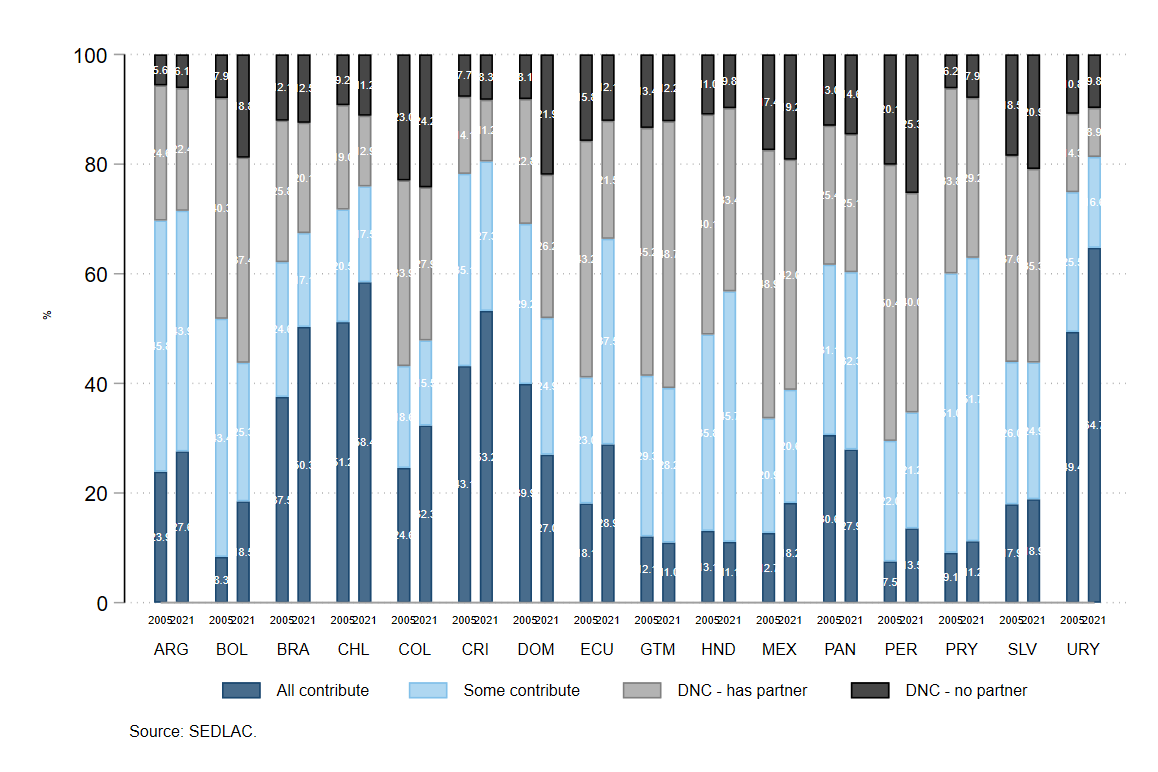
\includegraphics[scale=.45]{latex/figures/Household/snapshot_household_2005-2021.png}
    \label{fig:Household20052021}
    \justifying
    \footnotesize{Source: Household Surveys-SEDLAC.}
    \footnotesize{Note: Each bar is a weighted average of each country, weighting by total workers in 2005 and 2021.Data corresponds to 2021 except for Chile 2022, Guatemala 2014; Honduras 2019; Mexico 2018 and Uruguay 2019.}
    \footnotesize{Note: The figure reports the household contribution status to social security of households with at least one member works.   All contribute: corresponds to the percentage of households where all workers contribute to SS. Some contribute: corresponds to the percentage of households where some workers contribute to SS but not all. DNC – has partner: corresponds to the percentage of households where any worker contributes to SS, but the head of household have a partner. DNC – no partner: corresponds to the percentage of households where any worker contributes to SS, but the head of household do not have a partner.}
\end{figure}
\end{landscape}


\end{document}